\section{Results and Tests}
To test energy consumption during gameplay, the eAProfiler tool was used.

First, as can be seen in figure \ref{fig:nosleep},
the naive implementation is tested.
This version does not enter sleep mode after rendering a frame,
and contains no framebuffer rendering optimizations.

The high spikes (around $ 35 ma $ ) originate from when the
display buffer is refreshed (\emph{76800} system calls!). This implementation has an average
power consumption of rougly $ 33 ma $. Not very efficient.

\begin{figure}[H]
\centering
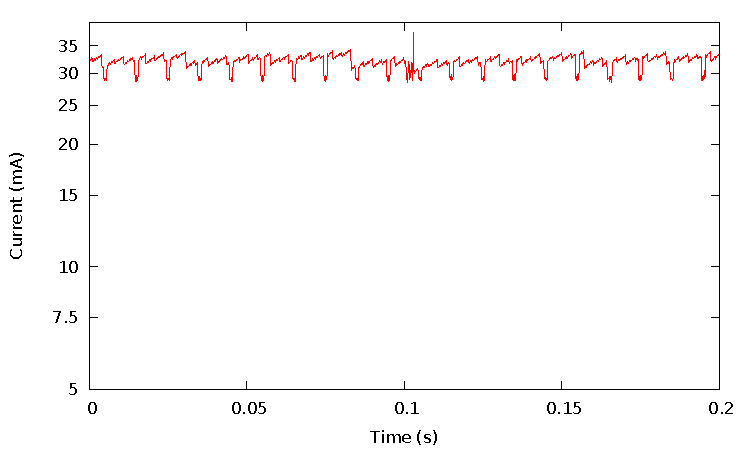
\includegraphics[width=0.7\textwidth]{figures/nosleep.pdf}
\caption{Graph of non sleeping code}
\label{fig:nosleep}
\end{figure}

The interesting thing to see is the comparison to figure
\ref{fig:sleep}, where the device goes to sleep after each
game loop iteration, only waking when it feels the time is
right to draw a new frame.

This version averages $ 29.01 mA $ when avake,
$ 7.59 mA $ when sleeping,
and $ 11.95 mA $ when averaged over 10 seconds.

The fat spikes are from when the framebuffer redraws.
The thin spikes are from kernel ticks,
these can be turned off for additional power savings.

\begin{figure}[H]
\centering
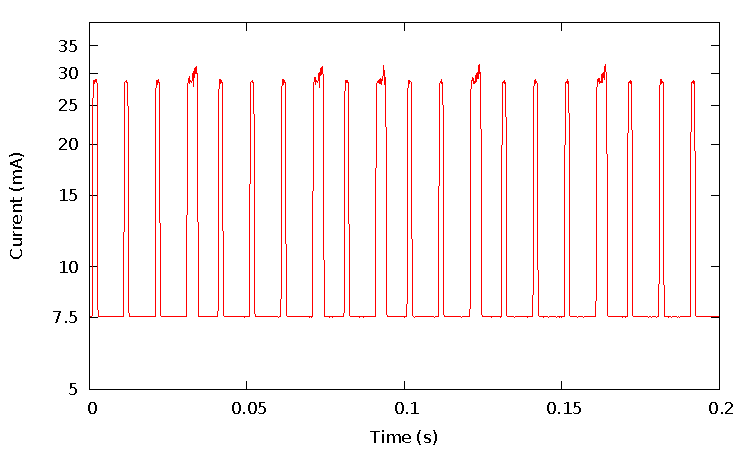
\includegraphics[width=0.7\textwidth]{figures/sleep.pdf}
\caption{Graph of sleeping code}
\label{fig:sleep}
\end{figure}

The power usage of the different implementations are nearly identical at the
peaks, but as shown in figure \ref{fig:sleep}, the energy savings are considerable.
